\chapter{Introduction}
%\addcontentsline{toc}{chapter}{Introduction}

	It has never been easier to capture visual information. Popular storage services grow lighting fast due to terabytes of photographs and movies we upload every day. The growth is so fast that hand-tagging and description, the traditional means of annotation, cease to suffice. They are ambiguous, emotional and rarely optimal. With no better solution at hand, databases are becoming increasingly harder to browse. Another but quite similar setting occurs in the field of mobile robotics. A mobile robot is there to interact with its environment. If so, it would be desirable for the robot to know what kind of surroundings it is in. The problem can be treated as a scene or object classification problem, one of the most popular computer vision issues in the last decade. As Forsyth and Ponce \cite{ponce2011cv} have it:
	
	\begin{quote} 
		computer vision is (...) an enterprise that uses statistical methods to disentangle data using models constructed with the aid of geometry, physics, and learning theory.
	\end{quote} 
	
	The area of computer vision is not new and have initially dealt with industrial inspection or mobile robot navigation. Recent applications include human-machine interfaces, medical diagnostics and image retrieval.
	
	This paper tackles two issues. Firstly, the Bag of Words (or BoW for short) approach to image classification is reviewed. The Bag of Words method has originated from the natural language processing domain \cite{tsai2012bag}. It makes a strong assumption that the word occurrence in a text document define the meaning of the document. It were Csurka \textit{et al} who have first used BoW for image classification in 2004 \cite{csurka2004visual}. Since we cannot simply translate an image into natural language a pipeline that help us achieve this goal is needed. It usually consist of: keypoint detection, feature extraction, vector quantization and classification, steps that will be discussed later.
	
	Secondly, a configurable and flexible application for point cloud classification is designed and implemented in C++. Many algorithms are suitable for the bag of words pipeline. To choose an optimal combination for a specific problem we have to perform extensive evaluation of those algorithms. The process can be greatly simplified by a programme that would be: (1) easily extensible, that is adding new algorithms wold be painless and (2) configurable, with every parameter (and algorithm) adjustable at runtime.
	
	The rest of this work is organised as follows: Section 1 summarises purpose and scope of this work. Section 2 describes the Bag of Words technique in detail. Construction of an image model is discussed and the most popular algorithms are outlined. Section 3 provides basic information on the problem of classification, introduces basic concepts and methods of classification. Section 4 names C++ computer vision and general purpose libraries used in this project. Finally, in Section 6 we describe two renown RGBD image datasets we have chosen to test our application at. The following chapters are titled ``Design'' and ``Experiments and Results''. The former analyses functionality of a programme for BoW object classification, its design and implementation details. The latter addresses the topics of experimental setup, performed experiments and a summary of results.
	
	\section{Scope and purpose of this work}
		The goal of this work is to design a flexible and configurable application for point cloud classification. The point cloud should be registered by the Microsoft Kinect RGBD camera. The scope of the work is as follows:
		\begin{itemize}
		\item literature review in the area of bag of words image classification
		\item design of a pipeline for bag of words classification of point clouds
		\item design of a configurable programme for point cloud classification
		\item implementation of the programme in C++ using OpenCV and/or PointCloud Library
		\item evaluation of algorithms for the bag of words classification
		\item evaluation of the programme on two scientific RGBD object databases
		\end{itemize} 
	
\section{Bag of Words}

	The Bag of Words model is a an intermediate representation used in natural language processing, information retrieval and data mining. The model can be seen as a simplification, for it obliterates any grammatical information and even word order contained within an original text document. What is left is an unstructured group of words, usually in a form of a vector or a histogram of word incidence.

	\begin{figure}[!ht]
	\centering
	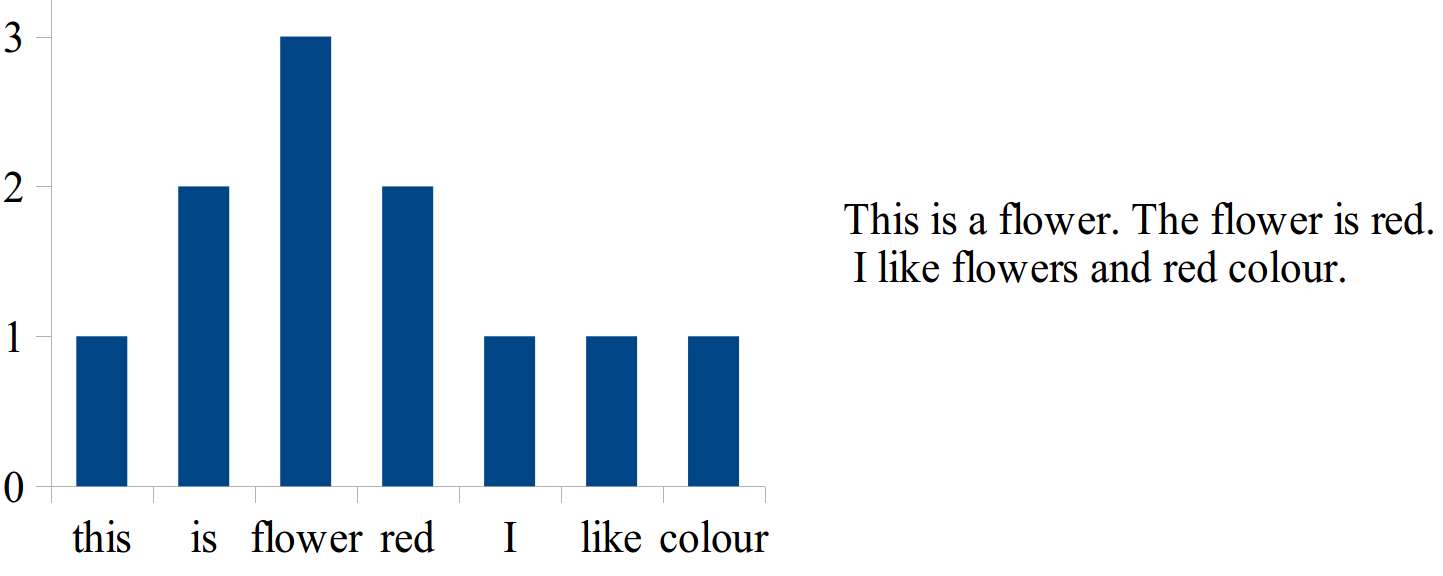
\includegraphics[width=0.7\textwidth]{../figs/bow_example}
	\caption{Bag of Words histogram}
	\label{fig:bow_example}
	\end{figure}
	
	The figure \ref{fig:bow_example} shows a piece of text and its BoW model, where articles and punctuation marks were left out. In order to compare different documents a global dictionary must be built. The dictionary (codebook) is constructed by taking every word from all available documents and removing duplicates. One can image that if a dictionary is of any considerable size resulting representation of especially small documents will be very sparse. Classification algorithms can be optimised for sparse data in order to boost performance.

	In natural language processing BoW is used to infer semantic meaning of documents. If we could translate an image into a text document we might be able to employ similar methods. A question arises: How does one make a text document from an image?

	\subsection{Processing Pipeline}	
	Tsai describes a well established pipeline that allows translation of images into text documents \cite{tsai2012bag}. It consists of the following steps: (1) region detection, (2) feature extraction, (3) vector quantization and (4) BoW histogram formation as can be seen in the figure \ref{fig:bow_pipeline}. The author summarises the most commonly used methods for performing these tasks. 
	
	\begin{figure}[!ht]
	\centering
	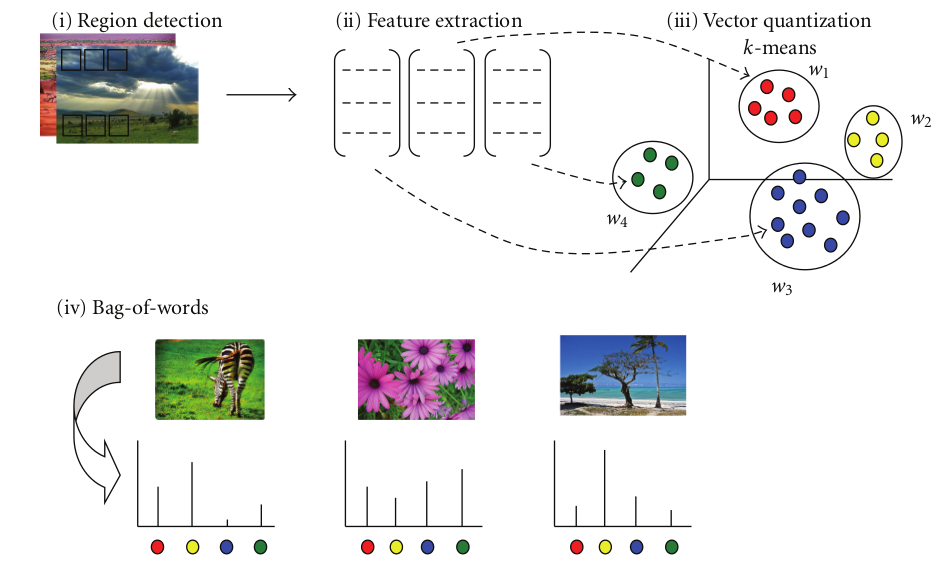
\includegraphics[width=0.75\textwidth]{../figs/tsai2012}
	\caption{Bag of Words pipeline. The figure comes from \cite{tsai2012bag}}
	\label{fig:bow_pipeline}
	\end{figure}
	
		\subsubsection{Region Detection}
		Characteristic region detection is the first step in any Bag of Words framework. Numerous detection methods have been developed, but choosing the right one for any particular case might prove tricky. 
		
		The most common detectors make use of a Harris corner detector or image's first or second derivatives. A Harris-Laplace detector is an example of a Harris-based detector. The Harris function is scale adapted and its outcome is a subject to a Laplacian-of-Gaussian (LoG) operator, which selects relevant points in scale space. Images' regions' 2\textsuperscript{nd} derivatives, namely the regions' Hessians, can be combined with a LoG operator as well. This combination allows selection of points significant in the two spaces: the scale space and the Hessian's determinant space. The latter entails the speed at which pixel intensities change in the neighbourhood of a point.	
	
		A number of more advanced recipes for salient region localisation have been developed and implemented. These include for example SIFT \cite{sift_keypoint}, SUSAN \cite{susan_keypoint} and Intrinistic Shape Signatures \cite{iss_keypoint}. The majority of keypoint detection formulas is being developed for the 2D domain. A number of them have been adapted to 3D, however. A comparative evaluation of detection algorithms available in the PointCloud Library (PCL, discussed below) can be find in \cite{pcl_keypoint_comparision}. Another comprehensive study is \cite{3d_keypoint_eval}. All these formulas, called sparse feature detectors, resort to selection of maxima in specific state spaces. An entirely different scheme is to use a dense feature detector. That is, take a uniformly sampled grid of points. Dense detectors have an advantage in that they sample slow changing regions in terms of gradient or hessian of an image. Examples of such regions would be a clear sky or a calm ocean. Li \emph{et al} showed that dense detectors generally outperform sparse ones \cite{fei2005bayesian}.
		
		\subsubsection{Feature Extraction}
		Suppose only coordinates of a keypoint were known. In case of even the smallest rotation or translation they would change and the keypoint would be lost. Keypoints should be described in a way that makes them invariant to affine transformations, changes in light intensity or colour saturation. It is hard to achieve all of these properties simultaneously, but methods that meet some of them exist.
		
		Keypoint description takes form of coordinates in a high-dimensional space. One of the most precise and repeatable algorithm is SIFT \cite{sift_features}, which is a 3D histogram of gradients structured as a 128-dimensional vector of floating point values. It is the most often extracted descriptor in BoW pipelines. Other methods include various colour descriptors, binary descriptors such as 512-dimensional GIST \cite{ponce2011cv}. There are techniques designed for 3D exclusively. Among them are Persistent Point Feature Histogram (PFH) \cite{pfh_rusu2008}, its faster alternative FPFH \cite{fpfh_rusu2009} and PFHRGB, which takes into account colour information, all implemented in PCL.
		
		\subsubsection{Vector Quantization}
		When features are extracted they have to be normalised. Vector quantization step have two main phases. The first one is a codebook construction from a training dataset. The second phase is responsible for parsing (or translation) raw image descriptors into a form compatible with the newly constructed codebook. The simplest way of building a dictionary is to find patterns or regions within the descriptors computed on a training dataset. Then, the parsing phase is about assigning a descriptor to one of the codebook elements (e.g. to one of the regions). Suppose we use centroids or medoids of the discovered regions as our codebook's entries. Then, we can match a descriptor to one of the centroids performing a nearest neighbour search. The descriptor parsed this way is called a \textit{visual word}. Finally, we build a histogram of visual word occurrence. The histogram have a fixed size equal to the codebook size. Each bin of the histogram tells us how many visual words of a particular kind were in the description of the corresponding image.
		
		The kMeans is the single most popular vector quantization algorithm used in the BoW pipelines \cite{tsai2012bag}. Developed in 1950's, it is well known and simple to implement. kMeans divides all data into a predefined amount of clusters and computes the clusters' centroids. Many modifications and alternative versions have emerged \cite{kmeans_jain2010data}. Some of them are: faster than the original \emph{approximate kmeans}, \emph{hierarchical kmeans}, which automatically chooses the final number of clusters and a \emph{soft kmeans} --- a variation of the algorithm that allows a fuzzy alignment. The fuzzy alignment mean that each point can belong to several clusters with different weights. A weight can be proportional for instance to the inverse square of the distance to a centroid. 
		
		If computational cost is of no concern, or if required precision is of the utmost priority, a Gaussian Mixture Model (GMM) can be used. The GMM partitions data into a set of clusters, finds their means and covariances. In the parsing step we compute a probability distribution of a descriptor over all the clusters. We can then build a fuzzy aligned histogram taking the probability distribution as weights. The GMM can be thought of as a generalisation of the kMeans algorithm. The drawback of the GMM is its massive computational cost in comparison with still expensive kMeans. Recently, Perronnin \textit{et al} proposed GMM based fisher-kernel vector quantization step with superior results \cite{fisher1, fisher2}.		
		
		After we choose a vector quantization algorithm, we have to decide what size of a dictionary to use. In a simplest case, when the kMeans is used, we can treat each clusters' centroid as a visual word. Therefore, the dictionary size defines how much information we retain in a BoW histogram. A big training set containing many classes with large inter-class and inter-class variance is likely to require a huge codebook. On the other hand, too big a dictionary might introduce quantization artefacts. One has to bear in mind that the vector quantization step is the most time-consuming part of the BoW pipeline. The highest computational complexity is associated with the codebook construction step and it is$O(n^3)$, where $n$ is the codebook size.		
		
		It is possible to combine several feature extraction algorithms before creating the codebook (Early Fusion) or create many codebooks and concatenate resulting histograms (Late Fusion). Both schemes are as simple as vector concatenation. The Early Fusion concatenates two feature vectors if they have been extracted from the same keypoint. The Late Fusion joins histograms, outputted by separate quantization steps.
	
	\subsection{Applications in Computer Vision}
	The Bag of Words approach is a tool than enables us to represent an image by a single feature vector of a chosen size. Its most popular applications in computer vision are Content Based Image Retrieval (CBIR) and Scene/Object Classification.
	
		\subsubsection{Content Based Image Retrieval}
		CBIR is a computer vision approach to image retrieval from large image databases. Tangelder \emph{et al} provides an overview of techniques applicable to 3D objects \cite{tangelder2008survey}. The task of image retrieval is to find a database entry that fulfil certain conditions. If we wanted to perform the task efficiently, we would have to meet the following criteria \cite{toldo2009bag}: (1) All entries should be indexed in a concise way, (2) a (dis)similarity measure should be provided and (3) an efficient search algorithm should be available. 
		
		Database entries (images) should be indexed beforehand. Otherwise we would have to compare all the entries explicitly. An index must be compact as well as discriminative. Suitable algorithms can be divided into three general categories: (1) feature based methods, (2) graph based methods and (3) other methods.

		Feature based methods can be further divided into global features and local features. The global features take form of a single vector (or a point in a \emph{d} dimensional space). They are usually associated with object's mass or volume or distributions of these. Being easy to compute and straightforward to implement, their discriminative power is rather low --- they cannot be used for partial matching, but are well suited for an early preprocessing. 
		
		Local features, on the other hand, describe object's characteristic regions. Their shape is similar to that of the global features, but instead of a single point in space there are multiple ones --- one for each considered region. Tangelder argues that local features based approaches are inefficient and lead to a complex indexing problem \cite{tangelder2008survey}. At the same time Toldo \emph{et al} and Li \emph{et al} show that Bag of Words local feature based approach has no such drawbacks. On the contrary --- it is easy to implement, efficient and provides state-of-the-art results.
		
		Feature based methods can be either local or global. Local features describe characteristic regions of an object, which have to be identified first. We have to carry out similar computation for each salient region. An outcome is a set of vectors, one vector for each region in \emph{d} dimensional space, where \emph{d} is dimensionality of the descriptor. Global features are generally easier (faster) to compute and more compact --- they take form of a single \emph{d} dimensional vector. Often global features are more computationally efficient and can be easily used for object indexing . Before the advent of BoW it was not clear how to use local features for indexing, nor there was any straight-forward dissimilarity measure available \cite{tangelder2008survey}. The Bag of Words approach solved these issues. What is more, it is easy to implement, efficient and provides state-of-the-art results \cite{li2010investigating}.
		
		\subsubsection{Scene and Object Classification}
		Scene and object classification are among the most popular issues of computer vision nowadays. We would like to perform those tasks automatically for the sake of surveillance, navigation or automatic image tagging. The very first attempt to use BoW in scene classification was made by Csurka \textit{et al} in 2004 \cite{csurka2004visual}. They were inspired by an idea of a ``texton'', a building block of texture introduced earlier in pattern recognition and texture classification. The authors suggested a BoW pipeline described above. Then, they fed the resulting BoW histograms into two classifiers: Support Vector Machine (SVM) and Na\`ve Bayes (both discussed below). Fei-Fei \emph{et al} refined the original approach by examining several keypoint detectors and descriptors \cite{fei2005bayesian}. Moreover, they developed a novel probabilistic graphical model for classification. They achieved accuracy of 76\% on a large 13 category dataset. 
		
		One of the best entries in an ILSVRC2013\footnote{\url{http://www.image-net.org/challenges/LSVRC/2013/results.php}} challenge, attempting to classify millions of images into 1000 categories, was submitted by a fisher vector based BoW approach as well. The top-5\footnote{top-5 --- the classification result is successful if the ground-truth category is in one of the five most probable categories predicted} accuracy rate was close to 85\%.
		
\section{Problem of Classification}

	To classify means to, given a set of categories, produce a category label for a given set of features \cite{ponce2011cv}. Image classification fits this description perfectly. The only difficulty lies in complexity of a raw image. Suppose we have a $320$ by $240$ three channel colour image. This amounts to a total of $230400$ dimensions, far too many to feed into any classifier directly. Fortunately, a Bag of Words histogram is a compact and discriminative intermediate representation that solves this issue. It can be used with any classifier. Classifiers can be two-class classifiers (e.g. binary) or multi-class classifiers. The latter are often a combination of several binary classifiers. The most popular classifiers are: k-Nearest Neighbours, Logistic Regression, Softmax Regression, Na\`ive Bayes and Support Vector Machine.
	
	\subsubsection{Na\`ive Bayes}
	Assume that we have a \textit{n}-dimensional feature vector $\mathbf{X}$ such that $\mathbf{X} = \left\{x_1, x_2, ... , x_\mathit{n}\right\}$ and an unknown category label \textit{C}. The probability of the category \textit{C} given the feature vector \textbf{X} is $P\left(\mathit{C}\middle|\mathbf{X}\right) = P\left(\mathit{C}\middle|\left\{x_1, x_2, ..., x_\mathit{n}\right\}\right)$. The strong (or na\`ive) Bayes assumption says that features are independent of each other, that is $P(\mathbf{X}) = P(x_1)*P(x_2)*...*P(x_\mathit{n})$. If so, we can compute probability distributions of every class in our training set given every feature. Then, for any new feature vector the joint probability distribution over a set of features can be calculated and an appropriate class label can be assigned.
	
	\subsubsection{k-Nearest Neighbours (kNN)}
	The nearest neighbours classifier assumes that if there are labelled points in a neighbourhood of a newly added point, then the new point can be classified based on it's neighbours' labels. There is an issue of choosing the correct number of nearest neighbours (or k) to consider.	
	
	\subsubsection{Support Vector Machine (SVM)}
	\begin{figure}[!ht]
	\centering
	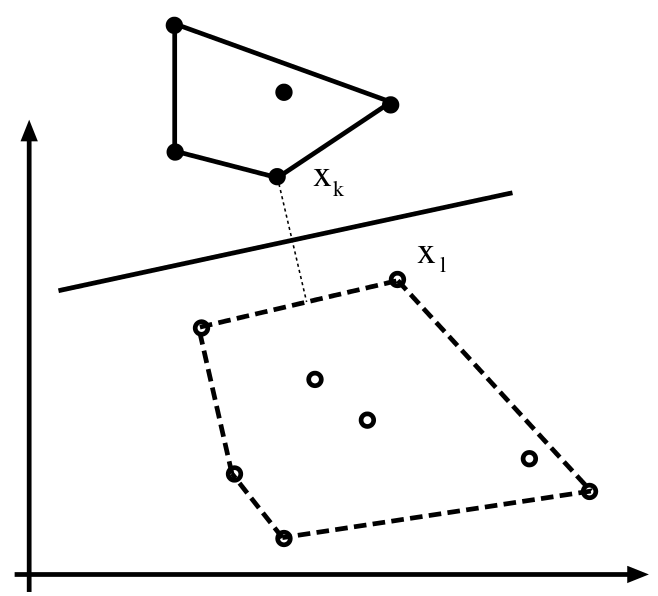
\includegraphics[width=0.75\textwidth]{../figs/svm}
	\caption{Classification by a Support Vector Machine. The distance of the separating plane from both datasets is maximal. The figure was originally published in \cite{ponce2011cv}}
	\label{fig:svm}
	\end{figure}
	
	Assume that a set of pairs $\{\{\mathbf{x}_1, y_1\}, \{\mathbf{x}_2, y_2\}, ...\}$ where $x_\mathit{i}$ are features and $y_\mathit{i} \in \{-1, 1\}$ are labels is given. Further assume that points with different labels are two linearly-separable datasets as shown in the figure \ref{fig:svm}, where dots and circles are points with different labels. Then, parameters \textbf{\textit{w}} and  \textit{b} exist such that	
	\begin{equation}	                        y_\mathit{i}\left(\mathbf{w}*\mathbf{x}_\mathit{i} + b\right) > 0
	\end{equation}
	for every $\mathbf{x}_\mathit{i}$ or a data point. This equation specifies constraints on a plane (or a hyperplane in general) that separates different classes. A Support Vector Machine finds the parameters \textbf{\textit{w}} and  \textit{b} so as to maximise the distance of the plane from members of both classes. We can combine several SVM classifiers in a 1-versus-all or an all-versus-all scheme.
	
\section{Libraries}

	We use the following third party C++ libraries:
	\begin{itemize}
	 \item Boost\footnote{\url{http://www.boost.org/}} --- of the biggest general purpose libraries
	 \item OpenCV\footnote{\url{http://opencv.org/}} --- a general computer vision library
	 \item PointCloud Library\footnote{\url{http://pointclouds.org/}} \cite{PCL} --- a library for point cloud processing
	 \item libsvm\footnote{\url{http://www.csie.ntu.edu.tw/~cjlin/libsvm/}} \cite{libsvm} --- a renown and very efficient SVM classifier implementation
	 \item Apache log4cxx\footnote{\url{http://logging.apache.org/log4cxx/}} --- Easy to use and intuitive logger
	\end{itemize}
	
	\subsection{Boost}
	Boost is a general purpose library available under the Boost Software License\footnote{\url{http://www.boost.org/LICENSE_1_0.txt}}. It is free for both commercial and non-commercial use. Boost comprises of more than 50 separate libraries. 12 of the most popular libraries have been incorporated into the new C++11 standard. Because of that, Boost may become redundant in many applications. The original library had contained conveniences such as smart pointers, multi-threading utilities and meta-programming tools. We excessively use smart pointers and meta-programming utilities; but the only package from the trimmed down Boost used in this project is the Boost.program\_options library. It enables convenient parsing of configuration files and command line arguments.
	
	\subsection{OpenCV}
	OpenCV is a general computer vision library available under the BSD License\footnote{\url{http://opensource.org/licenses/BSD-3-Clause}}. It is free for commercial and non-commercial use. It was designed for computational efficiency and real-time applications. OpenCV takes advantage of the underlying hardware employs hardware-specific optimisation e.g. SSE4. Some algorithms are written in nVidia CUDA and can use GPU for faster execution. Others use Threading Building Blocks (TBB, Intel's multithreading library) to enable concurrency. OpenCV is available for the most popular desktop and mobile platforms. It is written in optimised C and C++ and provides two interfaces: the original OpenCV 1.x C interface and a newer OpenCV 2.x C++ interface. This single library allows production of fully functional computer vision programmes. Many machine learning routines are available, too. Among them are: kMeans, Gaussian Mixture Model, Na\`ive Bayes, SVM, Random Forests and Boosting. We use OpenCV for input/output operations, image processing and vector quantization.
	
	\subsection{PointCloud Library}
	PointCloud Library (PCL) is a computer vision library suitable for point clouds processing, manipulation and visualisation. It is released under the BSD license and is free for both commercial and non-commercial use. PCL contains numerous state-of-the-art algorithms for feature detection, surface reconstruction, segmentation to name just a few areas. It is well documented and easy to use. Recently, a machine learning module containing SVM, kMeans and other algorithms. Some routines are multi-threaded thanks to the OpenMP library. A GPU module makes use of CUDA to lessen computation time. Unfortunately, the PCL is relatively new and its stability could be better. Currently available 1.7.1 version is going to be replaced by a soon-to-be-announced 2.0 version with incompatible API. In this project we try to build an application for point cloud applications. We extensively use PCL for operations like downsampling, keypoint detection, feature extraction.	
	
	\subsection{Apache log4cxx}
	Apache log4cxx is an efficient and easy to use logger for C++ programmes. It is based on a Apache log4j logger for Java applications. It provides a set of static methods for logging. It support simultaneous output to multiple destinations and have very well defined logging levels. It is perfectly documented as well.
	
\section{Datasets}

	Machine Learning algorithms provide a way of learning a function that maps input to the desired output. Classification algorithms require supervised training and labelled data. If we wanted to compare any algorithms we would have to do so on a common dataset. That is why multiple scientific datasets have been created: ImageNet\footnote{\url{http://www.image-net.org/}}, PascalVoc\footnote{\url{http://pascallin.ecs.soton.ac.uk/challenges/VOC/}}, LabelMe\footnote{\url{http://labelme.csail.mit.edu/Release3.0/browserTools/php/dataset.php}} and SUN\footnote{\url{http://groups.csail.mit.edu/vision/SUN/}} among others. Unfortunately, they contain RGB and grayscale images without any depth information. Therefore they cannot be used in this paper. On the other hand, the vast majority of RGBD datasets are focused on tracking or instance-level recognition. Others have very few categories or insufficient number of examples per category. We managed to find only two datasets suited to our needs. They are: the Berkeley 3D Object (B3DO) dataset \cite{B3DO} and a dataset compiled by Zhang \emph{et al} at the University of Tokyo\cite{zhangcategory}. The latter will be abbreviated Tokyo dataset from now on. 
	
	An interesting dataset is provided by the University of Washington \cite{dataset_washington}. It consists of video sequences that capture objects' round views in RGBD. Kinect Fusion\footnote{\url{http://msdn.microsoft.com/en-us/library/dn188670.aspx}} technology could be used to prepare excellent point clouds from the videos. We have decided against it, for a huge computational cost associated with this way of point cloud construction. Furthermore, in a real setting a mobile robot would have to circle an object in order to gather enough data.

	\subsection{Berkeley 3D Object Dataset}
	\begin{figure}[!ht]
	\centering
	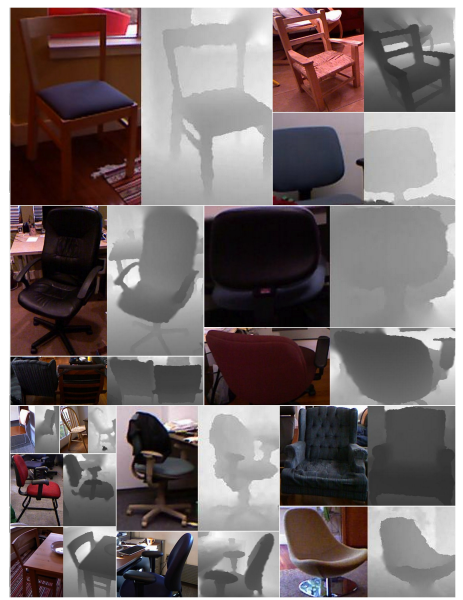
\includegraphics[width=0.5\textwidth]{../figs/b3do_dataset}
	\caption{Berkeley 3D Object Dataset. The figure comes from \cite{B3DO}}
	\label{fig:b3do}
	\end{figure}
	
	The Berkeley 3D Object dataset was specifically designed for the purpose of object detection and classification. It consists of cluttered images in indoor environment. There are around 50 classes with more than 20 examples in each of them. RGBD data are provided as pairs of colour images (8 bit RGB jpeg files) and depth maps (16 bit png files). Images are densely labelled --- for every pair of images there is an xml file with annotations. Each annotation states a category of an object as well as it's bounding box location. Images are cluttered, with many labelled and random objects per image. Labelled objects are often partially occluded. We do not address image segmentation nor object detection; we had to extract objects from the images before we could use the dataset.

	\subsection{The University of Tokyo Dataset}	
	\begin{figure}[!ht]
	\centering
	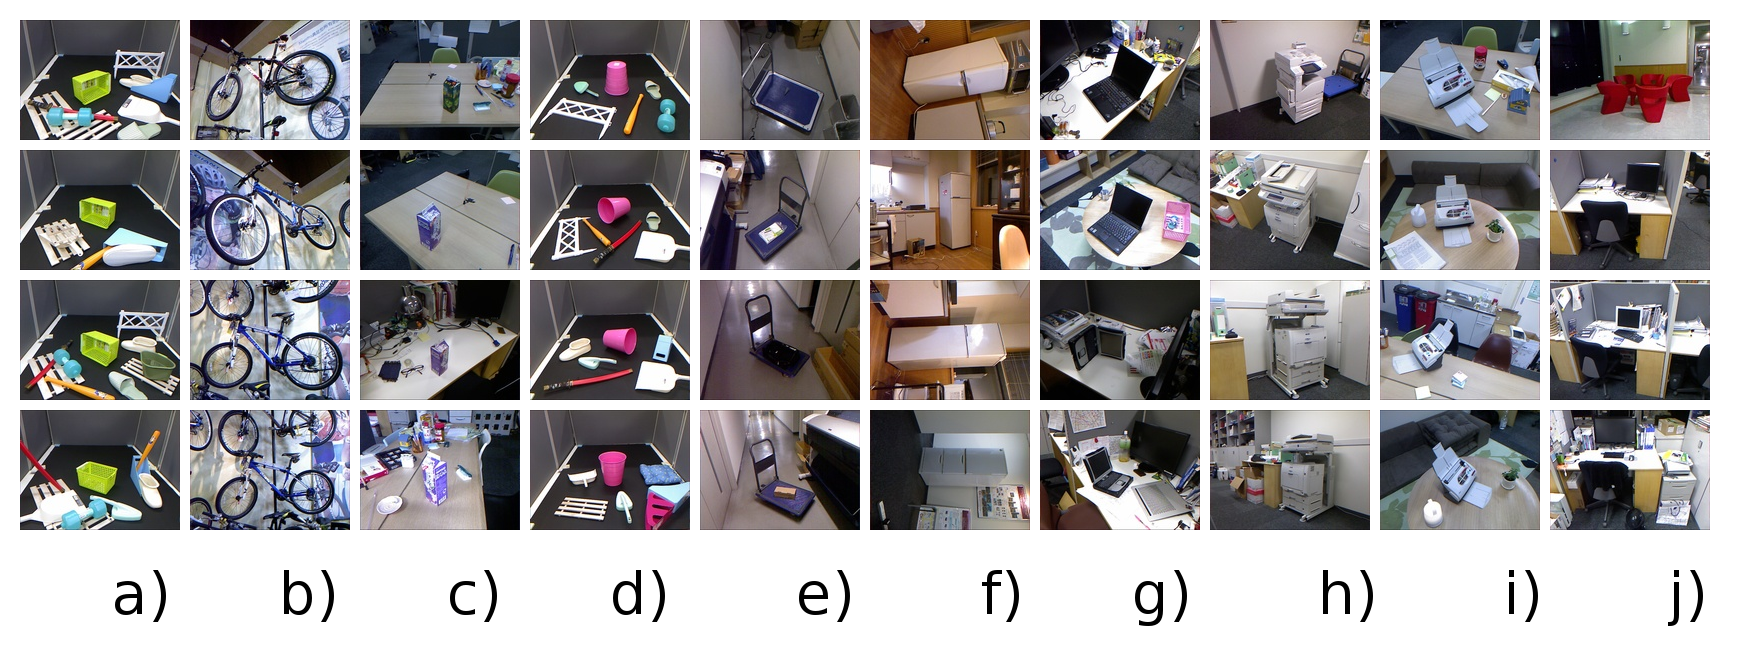
\includegraphics[width=1\textwidth]{../figs/tokyo_horizontal}
	\caption{The Tokyo dataset: a) basket b) bicycle c) box d) bucket e) cart f) freezer g) notebook h) printer i) scanner j) scene}
	\label{fig:tokyo}
	\end{figure}
	
	The Tokyo dataset is comprised of high quality images of objects in different settings, with changing viewpoint, object orientation and texture. The dataset is presented as colour images (8 bit RGB jpeg files) and depth maps (csv files with XYZ coordinates of each pixel).	This dataset is aimed at the task of object classification in casual images. There is one labelled object per image, without any bounding box given. Scenes are sometimes cluttered, with many random objects present at a scene.